  \begin{figure}[ht]
    \centering
    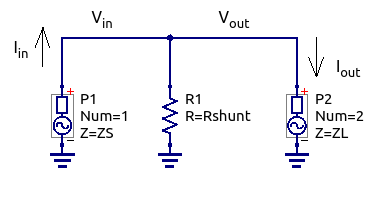
\includegraphics[width=10cm]{./images/r-shunt-attenuator-schematic.png}
    \caption{Shunt resistor attenuator}
    \label{fig:r-shunt-attenuator-schematic}
  \end{figure}

\noindent As in the case of the series resistor attenuator, the design equations can be derived from the loss caused by the impedance mismatch in the input and the output interfaces. Between the source impedance and the shunt resistor, the mismatch was found to be:

\begin{equation}
	t_1 = 1 - \left| \frac{Z_S - R \parallel Z_L}{Z_S + R \parallel Z_L} \right|
\end{equation}

\noindent Similarly, between the shunt resistor and the load impedance, the mismatch causes a insertion loss of:

\begin{equation}
	t_2 = 1 - \left| \frac{Z_S \parallel R - Z_L}{Z_S \parallel R + Z_L} \right|
\end{equation}

\noindent Consequently, the overall power loss is:

\begin{equation}
	t = t_1 \cdot t_2 = \frac{4 \cdot R^2 \cdot Z_S \cdot Z_L}{R^2 \cdot Z_L^2 + Z_S^2 \cdot (R^2 + 2 \cdot R \cdot Z_L + Z_L^2) + 2 \cdot Z_S \cdot Z_L \cdot R \cdot (R  + Z_L)}
	\label{eq:r-shunt-power-loss}
\end{equation}

\noindent As before, Eq. \ref{eq:r-shunt-power-loss} gives two solutions, but only one gives positive resistor values:

\begin{equation}
	R = Z_S \cdot Z_L \cdot \frac{2 \cdot \sqrt{Z_S \cdot Z_L \cdot \alpha^{n.u.}} + \alpha^{n.u.}  \cdot \left( Z_L + Z_S\right)}{4 \cdot Z_S \cdot Z_L - \alpha^{n.u.} \cdot (Z_L^2 + 2 \cdot Z_L \cdot Z_S + Z_S^2)}
\end{equation}